%% This is a skeleton file demonstrating the use of IEEEtran.cls (requires IEEEtran.cls version 1.8a or later) with an IEEE conference paper.
%%
%% Modified by Khan Reaz( kahn.reaz@ieee.org)
%% Support sites:
%% http://www.ieee.org/

%%***********************************************************
%% Legal Notice:
%% This code is offered as-is without any warranty either expressed or implied; without even the implied warranty of MERCHANTABILITY or FITNESS FOR A PARTICULAR PURPOSE! 
%% User assumes all risk and can modify as s/he wants.

%%***********************************************************

%package list
\documentclass[conference]{IEEEtran}
\usepackage{cite}
\usepackage{graphicx}
\graphicspath{ {images/} }



\begin{document}

%Here goes the title

\title{Concern Oriented Navigation Bar}


%Authors List

\author
{\IEEEauthorblockN{Author 1}
\IEEEauthorblockA{School of Electrical and\\Computer Engineering\\
University\\
Location\\
Email: }
\and
\IEEEauthorblockN{Author 2}
\IEEEauthorblockA{University\\
Location\\
Email: }
}
\maketitle


%Main body starts

\begin{abstract}
The advent of modeling in software engineering, like other engineering fields, has revolutionized the formalism and pace of software development. These models used at the different levels of abstraction during software development often relate and communicate among one another. A concern is a generic unit of reuse which groups related models (e.g., class diagrams, sequence diagrams, state machines) that cut across software application. However, in concern oriented reuse and other software development paradigms, little or no attention has been drawn on these related models are navigated both internally (intra model navigation) and externally (inter models navigation). This paper aims to establish an easy-to-use and streamlined mechanism of navigation among related model artifacts. Our navigation mechanism is augmented with different colors indicating where a model element (to-elements) are located. Our findings will improve the development of concerns and other software application which involves related models.
\end{abstract}


\begin {IEEEkeywords}
Navigation. Bars, Concerns, Reuse.
\end{IEEEkeywords}

 
\section{Introduction} \label{intro}
{O}{wing} to the advent of model driven engineering \cite{brambilla2012model,schmidt}, virtually all software artifacts can be represented as models. In software development, models play important roles including abstraction and simplified representation of software products. A lot of efforts have been posited on to improve the use of models in software development which includes but not limited to reuse of models, domain specific modeling language, and visualization of models. In Concern Oriented Reuse (CORE), a typical example of model reuse, several models that cut across software application are grouped together to ease the reuse of models \cite{alam2013concern2}. In software product lines, different model artifacts are grouped with commonality and variability which improves the development of each product in the family of the products \cite{spl}.

While great efforts have been posited to augment the communication among these related model artifacts, the mechanism to traverse the model elements has not received an adequate attention. In this paper, we address this problem by presenting a navigation bar which aims to enable software developers traverse among different model elements with ease. We further support the with colour highlighting. i.e., a model element selected to be navigated to will be highlighted with colour for easier identification. We believe that this proposition will reduce time spent during software development and make development more friendly.

\section{Background} \label{background}
In this section, we briefly present Concern Oriented Reuse (CORE) which we use to demonstrate our navigation bar. CORE is a software reuse paradigm that promotes the use of concern as its main artifact during software development. A concern groups related models (e.g., class diagrams, sequence diagrams, state machines) that cut across software application, and provides three interfaces to facilitate reuse: the variation, customization, and usage interfaces. The details of the interfaces is out of scope in this paper.  During software reuse, different realization models are \textit{woven/composed} to produce a specific application required for a given a context or domain. During concern development, it apparent that the developer wants to navigate different models of a concern. The ease and improved mechanism to navigate these models form the fulcrum of this paper. In the next section, we give a structural overview of a concern and then present the navigation bar mechanism.

\subsection{Concern Structure}
The basic structure of a concern is shown in the excerpt of the metamodel in Figure \ref{fig : core metamodel}. A concern (\textit{COREConcern}) groups related models (\textit{COREModel}) together, with at least one model by default. A COREModel is an abstract class which is concretely defined via sub-classing (\textit{corification}). Several models including class diagram, sequence diagram, state machine, and aspects can be corified, i.e., making them to behave like concern models (\textit{COREModel}).  A concern is composed of one feature model (\textit{COREFeatureModel}), see Figure \ref{fig : core metamodel}, a subclass of COREModel. A feature model groups the commonality and variations of a family of software products such as authentication, logging, and authorization. Each software artifact in a family is represented as a feature (\textit{COREFeature}). A feature is realized by one or more COREModels, conversely, a COREModel can realize one or more core features. The classes with pink background in Figure \ref{fig : core metamodel} depicts the structure through which concern models are reused, which is not the main focus of this work.

\begin{figure}
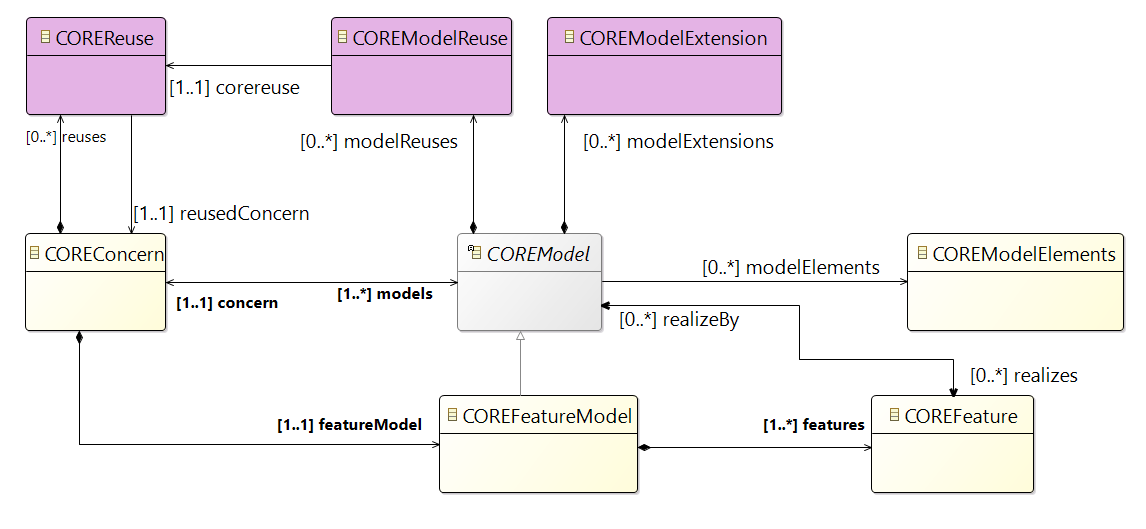
\includegraphics[width=\linewidth]{coremetamodel.PNG}
	\caption{Basic Structure of a Concern}
	\label{fig : core metamodel}
\end{figure}

\section{Section 2}
\label{section2}

  
  
	\subsection{IoT}
	 
	 	 
	 

	
	


\section{Section 3}
\label{section3}


\section{Section 4}
\label{section4}
   
%example for Bullet point list

\begin{itemize}
\item example
\end {itemize}



%example for numbered list
    \begin{enumerate}
    \item example
 
    \end{enumerate}
    

    

%example for inserting image
\begin{figure}[h]
   \centering
   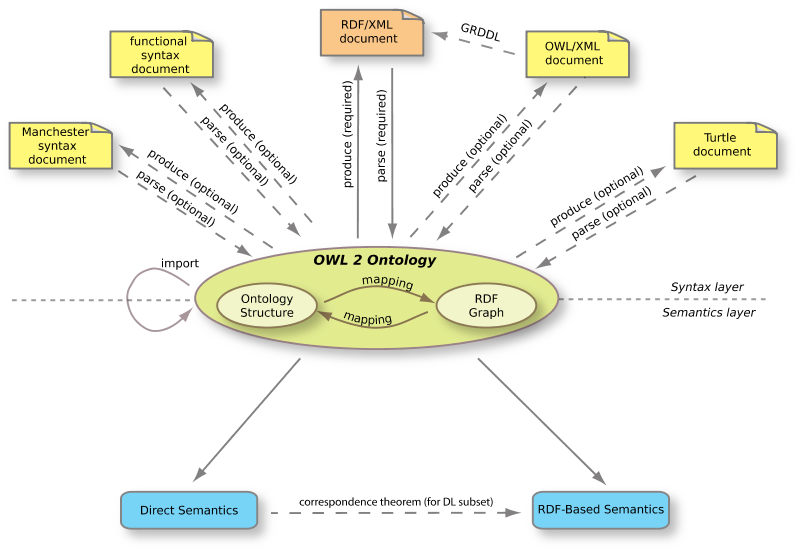
\includegraphics[scale=.45]{OWL2}
    \caption{The structure of OWL2}
    \label{fig:OWL2}
\end{figure}


	
	
\section{Conclusion}
\label {conclusion}
\input{sections/5_conclusion.tex}


\bibliographystyle{IEEEtran}
\bibliography{bibliography}

\end{document}